\section*{Methods}

This study proposes a comprehensive and systematic procedure for classifying Vietnamese speech commands using the ConvMixer architecture \cite{trockman2022patchesneed} in the audio domain. The focus lies in optimizing both input feature quality and architectural efficiency, while establishing a controlled and statistically robust comparison protocol across multiple lightweight models.

Figure~\ref{fig:novelty} illustrates the conceptual novelty of adapting the ConvMixer architecture to the audio domain using Mel-spectrogram representations. As shown on the left, the input Mel-spectrogram encodes time–frequency energy patterns of speech signals, which are treated as a two-dimensional structure analogous to an image. The spectrogram is first partitioned into local patches, enabling patch-level feature abstraction while preserving the inherent temporal–spectral structure of audio signals.

\begin{figure}[htbp]

\centering

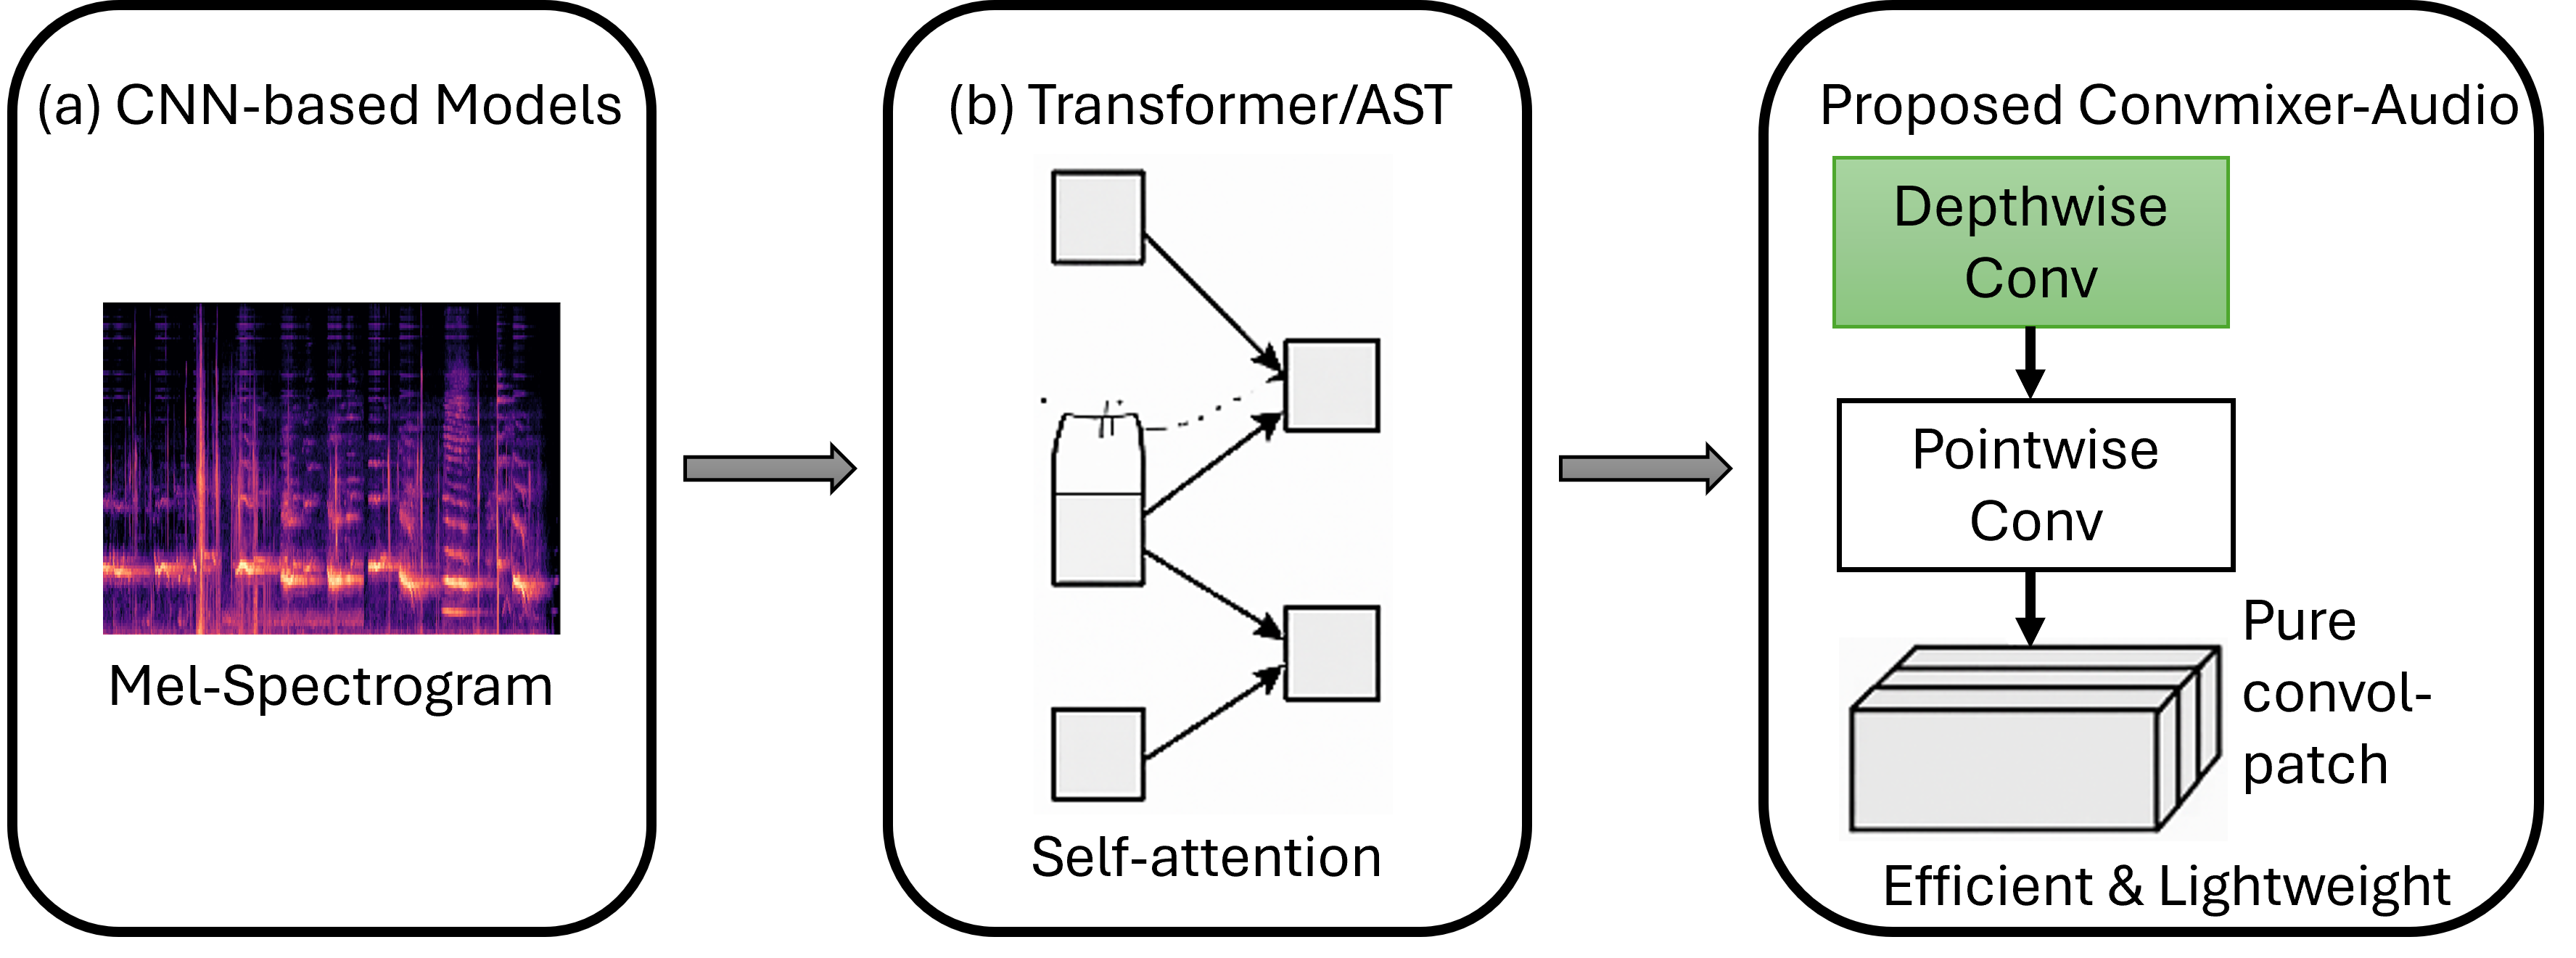
\includegraphics[width=0.8\linewidth]{imgs/Convmixer-novelty.png}

\caption{\label{fig:novelty}Conceptual diagram of ConvMixer audio novelty}

\end{figure}

Unlike attention-based or MLP-based patch models, the proposed ConvMixer-Audio framework performs feature mixing exclusively through convolutional operations. Specifically, depthwise convolution is employed to capture spatial relationships within each patch across the time–frequency plane, effectively modeling local and mid-range temporal–spectral dependencies. Subsequently, pointwise convolution enables channel-wise feature interaction, facilitating global feature integration across patches.

This convolution-only patch-based design eliminates the need for self-attention mechanisms while retaining the representational benefits of patch processing. As a result, ConvMixer achieves a favorable balance between expressive capacity and computational efficiency, highlighting its suitability for lightweight, deployable speech understanding systems in edge-AI and embedded environments.


\begin{figure}[htbp]

\centering

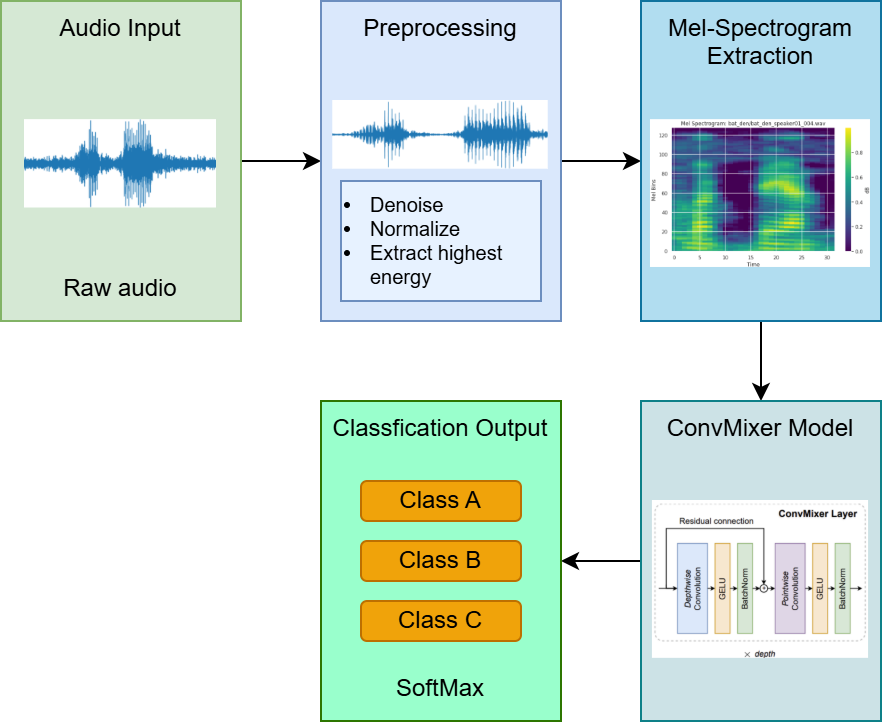
\includegraphics[width=0.8\linewidth]{imgs/fig1.png}

\caption{\label{fig:overview}Overview of the proposed audio classification framework. The pipeline includes raw audio input, preprocessing (denoising, normalization, and energy-based segmentation), Mel-spectrogram feature extraction, ConvMixer-based model training, and final classification using the Softmax layer}

\end{figure}



\subsection*{Audio Preprocessing}

A refined preprocessing pipeline was designed to produce standardized, noise-reduced, and energy-balanced one-second speech segments for Mel-spectrogram extraction. Compared with the baseline version, this workflow introduces two key enhancements—Voice Activity Detection (VAD) and a two-stage high-energy segment extraction—substantially improving the quality and consistency of speech features for lightweight ConvMixer models. Figure~\ref{fig:overview} presents an overview of the proposed end-to-end audio classification framework based on the ConvMixer architecture. The pipeline begins with raw audio input, which undergoes a dedicated preprocessing stage including denoising, amplitude normalization, and energy-based segmentation to ensure consistent and informative speech segments. These operations aim to suppress background noise, remove silence, and standardize signal amplitude, thereby improving the robustness of downstream feature extraction.

The pipeline begins by loading the raw recordings, converting them to mono, and resampling at 16~kHz to retain the 0–4~kHz speech band while reducing data size. Spectral noise reduction is then applied using subtraction or gating in the frequency domain to suppress background interference and enhance clarity.

Voice Activity Detection (VAD) is performed using Google’s WebRTC algorithm~\cite{WebRTCVAD}, which analyzes 30~ms frames and removes non-speech intervals. A sensitivity level of~2 offers a balanced trade-off between preserving speech and eliminating silence or background noise.

Next, a two-stage high-energy extraction ensures consistent and content-rich inputs. A 1.5-second sliding window (stride 0.3~s) first identifies the segment with the highest total energy, followed by a finer 1-second search (stride 20~ms) within that region to locate the most informative sub-segment. This hierarchical approach captures the most relevant portion of each utterance while standardizing duration.

Finally, peak normalization scales each waveform to a uniform amplitude, with the maximum absolute value set to~0.99 of the dynamic range and converted to 16-bit integer format. The resulting one-second segments are noise-suppressed, amplitude-normalized, and rich in speech information, providing stable and high-quality inputs for Mel-spectrogram feature extraction. Figure~\ref{fig:preprocessing} illustrates the complete preprocessing flow.

\begin{figure}[htbp]
\centering
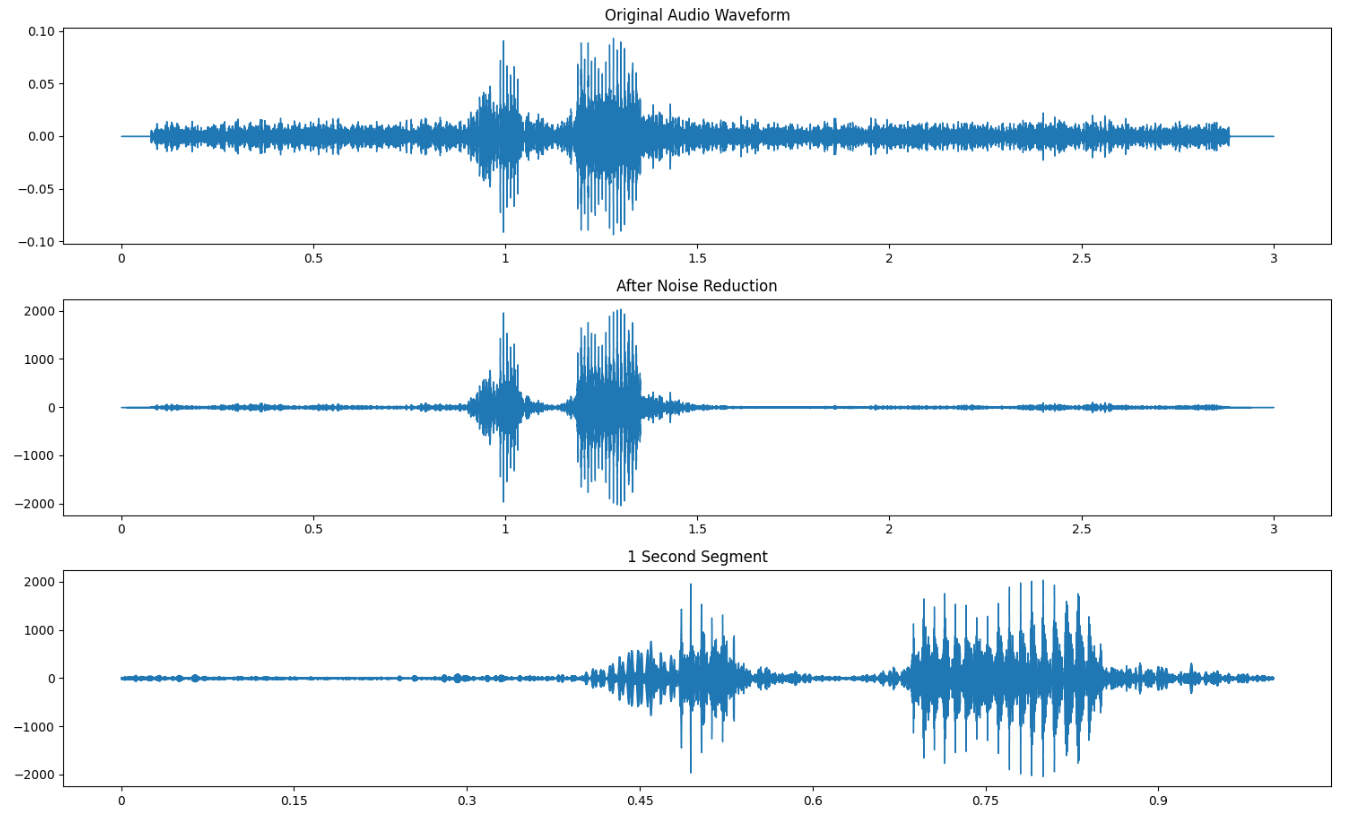
\includegraphics[width=0.75\linewidth]{imgs/fig2.png}
\caption{\label{fig:preprocessing}Overview of the audio preprocessing pipeline. The raw waveform undergoes denoising, voice activity detection (VAD), normalization, and segmentation into 1-second clips before feature extraction.}
\end{figure}



\subsection*{Mel-spectrogram Feature Extraction}

The input feature for the ConvMixer model is the Mel-spectrogram, a 2D representation aligned with human auditory perception on the Mel scale~\cite{Stevens1937MelScale}. The extraction parameters were configured as follows\cite{mcfee2015,Park_2019}:

\begin{itemize}

\item \textbf{STFT parameters:}  
The window size ($n\_fft = 2048$) and hop length ($hop\_length = 128$) were selected for fine-grained temporal resolution. With a 16~kHz sampling rate, each frame corresponds to 0.008~s, suitable for short speech events.  
The Short-Time Fourier Transform (STFT) converts overlapping time-domain frames $x[n]$ into their frequency components using a Hann window:
\[
X(f, t) = \sum_{n=0}^{N-1} x[n] w[n - t \cdot hop\_length] e^{-j 2 \pi f n / N}.
\]

\item \textbf{Mel parameters:}  
A 128-band Mel filter bank was applied, covering 20–8000~Hz (the Nyquist range). The Mel scale mapping is:
\[
m = 2595 \log_{10}\left(1 + \frac{f}{700}\right),
\]
which provides higher resolution at perceptually important low frequencies.

\item \textbf{Conversion and normalization:}  
The power spectrum was computed as $P(f, t) = |X(f, t)|^2$ and filtered by triangular Mel filters $W(m, f)$ to produce the Mel power spectrum:
\[
P_{\text{Mel}}(m, t) = \sum_f W(m, f) \cdot P(f, t).
\]
It was then converted to the logarithmic scale:
\[
\text{Mel-spectrogram (dB)} = 10 \log_{10}\left(\frac{P_{\text{Mel}}}{P_{\text{ref}}} + \epsilon\right),
\]
with $\epsilon = 10^{-10}$ ensuring numerical stability.  
Finally, Min–Max normalization was applied:
\[
X_{\text{norm}} = \frac{X - X_{\min}}{X_{\max} - X_{\min}},
\]
producing values in the $[0, 1]$ range for consistent model input.

\end{itemize}

The resulting Mel-spectrograms were resized to a fixed dimension of $128 \times 32$ (128 Mel bins, 32 time frames) using bilinear interpolation and stored as \texttt{.npy} files for model training. All feature extraction steps (STFT computation, Mel filtering, log compression, and normalization) were implemented using Librosa and Torchaudio to ensure consistent and reproducible spectrogram generation across experiments\cite{mcfee2015,Park_2019}. Additionally, SpecAugment-based masking operations were incorporated as part of the data augmentation pipeline\cite{Park_2019}.

\begin{figure}[htbp]
\centering
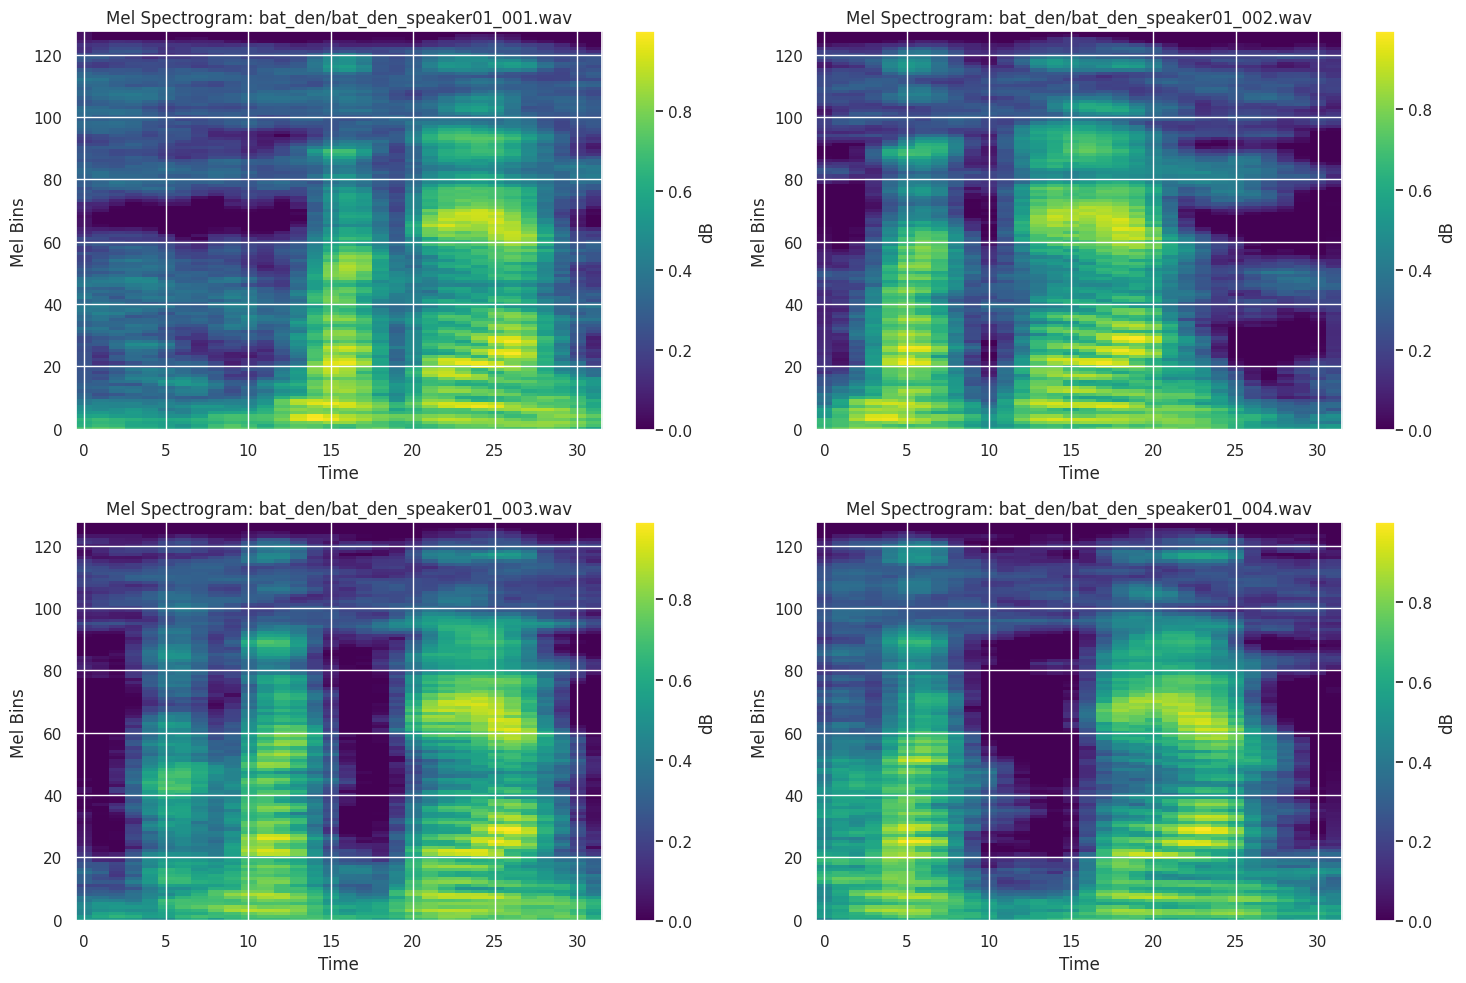
\includegraphics[width=0.75\linewidth]{imgs/fig3.png}
\caption{\label{fig:melspec}Example Mel-spectrograms of four “bat\_den” (turn-on light) samples after preprocessing. The time–frequency patterns highlight energy concentration across specific bands.}
\end{figure}


\subsection*{Data Augmentation}

To enhance model robustness and mitigate overfitting on the relatively small dataset (1,853 samples), state-of-the-art data augmentation techniques were applied only to the training set. Time Masking was applied with a 50\% probability, randomly covering up to 10\% of the time dimension. Frequency Masking was also applied with a 50\% probability, randomly covering up to 10\% of the Mel bins. Furthermore, Time Stretching was used with a 50\% probability, altering the playback speed between 80\% and 120\% of the original duration via linear interpolation, before resizing the feature back to the original dimensions of 128 × 32 \cite{Cubuk2020RandAugment, Zhang2017Mixup, Yun2019CutMix, Zhong2020RandomErasing}.

\subsection*{ConvMixer Architecture}

The ConvMixer architecture was employed for its simplicity and parameter efficiency, operating on a patch representation similar to ViT and MLP-Mixer but utilizing only standard convolutions for both spatial and channel mixing \cite{trockman2022patchesneed, dosovitskiy2020image, Tolstikhin2021MLPMixer}. Unlike attention-based models, ConvMixer preserves convolutional inductive biases such as spatial locality and translation equivariance while retaining the patch-based abstraction of vision transformers.

The implemented model follows the ConvMixer-256/8 configuration, where the hidden dimension ($dim = 256$) and depth ($depth = 8$) define the number of feature channels and repeated mixing blocks, respectively. This setting results in approximately 0.72 million trainable parameters, striking a balance between expressive capacity and computational efficiency. Preliminary ablation trials with smaller (ConvMixer-128/8) and deeper variants (ConvMixer-256/12) revealed that ConvMixer-256/8 offered the best trade-off between accuracy and model complexity, avoiding overfitting while maintaining fast convergence.

\begin{itemize}
\item \textbf{Patch Embedding:} The single-channel input ($1 \times 128 \times 32$) is transformed into 256-channel patch embeddings through a convolutional stem:
\begin{equation*}
X_0 = \text{GELU}(\text{BN}(\text{Conv}_{7\times7,\,stride=7}(X))),
\end{equation*}
where $\text{Conv}_{7\times7}$ extracts local structures within each patch while downsampling the feature map by a factor of 7 in both dimensions.

\item \textbf{ConvMixer Blocks:} Each of the $L=8$ repeated blocks performs spatial and channel mixing:
\begin{align*}
Z' &= X + \text{GELU}(\text{BN}(\text{DWConv}_{9\times9}(X))), \\
X' &= \text{GELU}(\text{BN}(\text{Conv}_{1\times1}(Z'))),
\end{align*}
where $\text{DWConv}$ denotes depthwise convolution (grouped by $dim$). The residual connection maintains gradient stability and preserves low-level information, while the $(1\times1)$ convolution enables full cross-channel interaction analogous to MLP mixing layers.

\item \textbf{Output Head:} The final feature map is globally aggregated via adaptive average pooling:
\begin{equation*}
y = \text{Linear}(\text{Flatten}(\text{AvgPool}(X_L))),
\end{equation*}
producing 13 class logits corresponding to the target categories.
\end{itemize}

Overall, the ConvMixer architecture can be summarized as a hierarchical composition:
\begin{equation*}
f(X) = \text{Linear}(\text{AvgPool}(\text{MixBlock}_L(\dots \text{MixBlock}_1(\text{PatchEmbed}(X))))),
\end{equation*}
where $\text{MixBlock}_i$ alternates between spatial and channel mixing. This compact yet expressive design retains the representational power of deep convolutional models while maintaining computational efficiency, making it well-suited for real-time and embedded speech recognition tasks.


\subsection*{Training Configuration}

\subsubsection*{Dataset Split}
The dataset of 1,853 Vietnamese speech command samples was divided using a stratified split to maintain class balance across subsets: 75\% for training (1,385 samples), 15\% for validation (274 samples), and 10\% for testing (194 samples). Each subset preserves proportional representation of all 13 classes. This split policy was fixed and shared by all compared architectures.

\subsubsection*{Optimization Settings}
Training was performed using the Adam optimizer with an initial learning rate ($lr = 0.001$) and weight decay ($1 \times 10^{-4}$) for L2 regularization \cite{Loshchilov2018AdamW}. The batch size was set to 32, and the CrossEntropyLoss function was applied for multi-class classification.

\subsubsection*{Learning Rate Scheduling}
A $ReduceLROnPlateau$ scheduler was used to automatically adjust the learning rate, operating in \textit{‘max’} mode to monitor validation accuracy. The learning rate decayed by a factor of 0.2 if no improvement was observed for 3 consecutive epochs, with a minimum learning rate threshold of $1 \times 10^{-6}$.

\subsubsection*{Regularization and Early Stopping}
To prevent overfitting, Early Stopping was employed with a patience of 5 epochs and a minimum required improvement ($min\_delta = 0.02$) in validation accuracy. The maximum training duration was capped at 25 epochs, balancing computational efficiency and model stability.

\subsubsection*{Controlled Baseline Protocol}
To address fairness concerns in cross-model evaluation, we define a controlled benchmark in which ConvMixer-256/8, ResNet-18, MobileNetV2, EfficientNet, and AST (tiny configuration) are trained on exactly the same dataset split, with identical preprocessing, Mel-spectrogram extraction settings, augmentation strategy, optimizer family, early stopping policy, and epoch budget. This design isolates architectural effects and avoids confounding factors caused by inconsistent pipelines.

For the ResNet baseline, we adopt a standard ResNet-18 configuration adapted to spectrogram input by setting the first convolution to one input channel and replacing the classification head with a 13-class output layer.

For the transformer baseline, we use the official AST implementation (\url{https://github.com/YuanGongND/ast/}) with a tiny configuration (reduced embedding width and depth) \cite{Gong2021AST} so that training cost remains comparable to lightweight convolutional baselines while preserving the core patch-embedding and self-attention mechanism.

\subsubsection*{Multi-seed Statistical Evaluation}
To improve result reliability on a relatively small dataset, each model is trained with five random seeds: 42, 43, 44, 45, and 46. For each metric (Accuracy, macro-F1, weighted-F1, and loss), we report mean$\pm$std across seeds. We additionally compute a 95\% confidence interval for the mean when needed:
\[
\mathrm{CI}_{95\%} = \bar{x} \pm 1.96\frac{s}{\sqrt{n}}, \quad n=5.
\]
This protocol reduces dependence on a single random run and provides a more stable basis for model comparison.
